% -----------------------------------------------
% Vlastní text práce (kapitoly práce)
% -----------------------------------------------

% -----------------------------------------------
\chapter{Gamma rays detection}
% -----------------------------------------------


% -----------------------------------------------
\section{Properties and parameters of detectors}
% -----------------------------------------------
The main parameters which are crucial for purposes of Mössbauer are detection efficiency and energy resolution at low gamma energies.
\par
Nowadays three main types of detectors are employed on the field of nuclear physics - gas, scintillation and semiconductor.
The Mössbauer spectrometer setups in laboratories of KEF are usually based on gas or scintillation detectors.


\subsection{Gas proportional detectors}
The gas detectors are usually tubes with electrodes filled with a special gas mixture. The incoming particle ionizes the gas, creating free ions and electrons.  According to the applied voltage, the gaseous detector can be operated in proportional regime, which is characterized by additional multiplication of charge carriers and thus, the signal can be amplified. The advantage of gaseous detectors is that they offer good energy resolution, but on the other hand their detection efficiency is low mainly due to the fact, that the gas density is small. Count rates are also affected by the long duration of the ionization effect. For operation they require high voltages (usually over 1000 V) and in case of flow counters they also require pressure cylinders along with other heavy equipment. 

%\begin{figure}[H]
% \centering
% 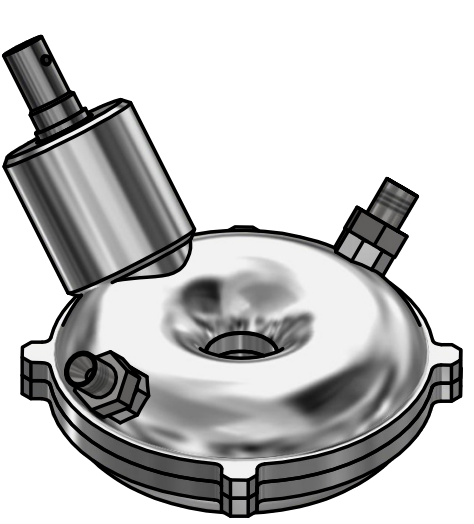
\includegraphics[scale=0.55, angle = 0]{./pictures/GASdet.png}
% \caption{Toroidal proportional gas flow counter used in MS spectrometer \cite{Optimized}.}
% \label{toroid}
% 
%\end{figure}


\subsection{Scintillation detectors}
By scintillation detector is usually meant a scintillation crystal coupled with a photomultiplier tube (PMT). The first conversion happens inside the scintillation crystal, where the incoming particle generates number of photons linearly dependent on its energy. These photons are captured by PMT's photo-cathode, where are they converted into electrons, and then multiplied on PMT's dynodes. This amplification requires high voltages around $1000 - 2000$ V. The internal amplification inside PMT can be around $10^6$.
\par
The detection efficiency is very high and due to the short duration of excitation effects, they can be used at high count rates.
\par
However, their energy resolution is much worse than in case of gases and semiconductors. The gamma spectra obtained this way usually have distorted wide peaks, which negatively affects Mössbauer spectrometry. The PMTs also cannot be employed inside the magnetic fields. 


\subsection{Detectors based on semiconductors}
The semiconductors offer the best energy resolution and a very good efficiency, however, they are usually more expensive than the other types of detectors. They can be used as direct radiation detectors (more often) or there is also a possibility to couple them with a scintillator crystal. 
\par
One problem with semiconductor detector is that there is no internal amplification, so the signals coming out of the detectors have to be strongly amplified by electronics.
However, they are small and compact. They also don't require high voltage sources or heavy pressure cylinders to operate. These facts are crucial if it comes to making more compact Mössbauer spectrometers. The Mössbauer spectrometer MIMOS II \cite{https://doi.org/10.1029/2003JE002138} based on 4 Si PIN diodes was a part of two rowers Spirit and Opportunity on their mission on Mars. 




% %%%%%%%%%%%%%%%%%%%%%%%% End of file %%%%%%%%%%%%%%%%%%%%%%%%